\section{Demo}\label{Demo}

\subsection{Kinetic Energy Example}\label{Kinetic}

\begin{figure*}[t]
  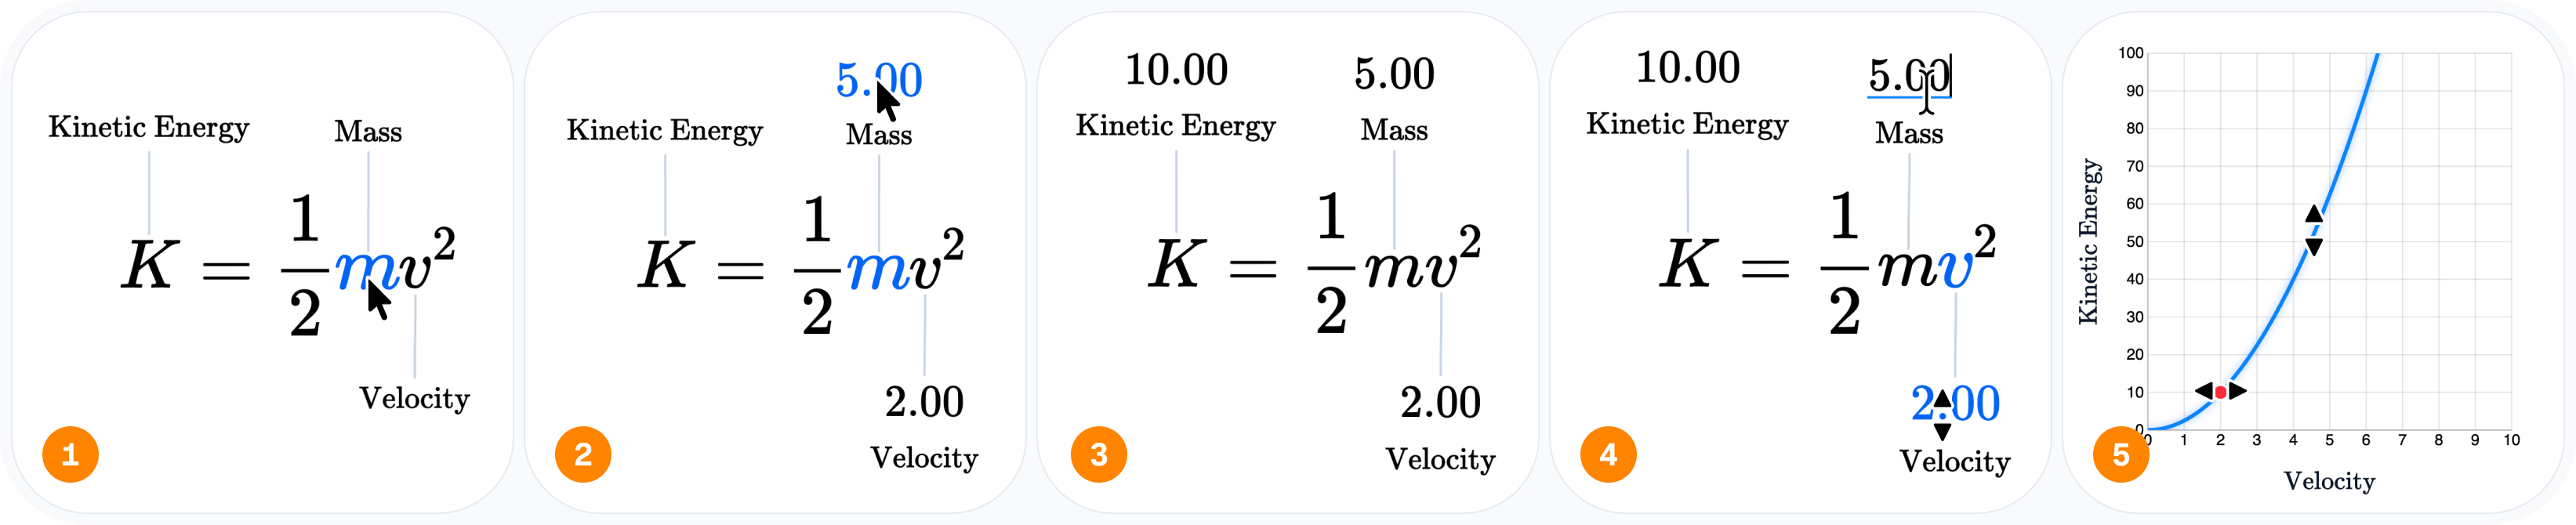
\includegraphics[width=\textwidth]{fig/demo-1.png}
  \caption{Kinetic energy authoring workflow. (1) Declaring variables adds labels. (2) Default values populate them. (3) Semantics compute derived variables. (4) Input modes enable drag and inline editing. (5) A graph entry creates a bidirectional plot.}
  \label{fig:demo-1}
\end{figure*}

Liv is writing a passage about the kinetic energy formula $K = \frac{1}{2}mv^2$. She wants to create an interactive version showing how changes in mass and velocity affect kinetic energy, linked to a synchronized visualization. Instead of writing hundreds of lines of UI code or combining separate math and diagramming packages, Liv imports Delta into her TypeScript file and creates a configuration:

\begin{tcolorbox}[codebox]
\begin{lstlisting}[style=jsstyle]
const kineticConfig: Config = {
  formulas: [
    id: "kinetic-energy", latex: "K = \\frac{1}{2}mv^2",
  ],
  variables: {
    K: { name: "Kinetic Energy" },
    m: { name: "Mass", default: 5 },
    v: { name: "Velocity", default: 2 },
  },
}
\end{lstlisting}
\end{tcolorbox}

To render the formula, Liv places a \texttt{Formula} component inside a \texttt{Provider} that supplies the Delta context:

\begin{tcolorbox}[codebox]
\begin{lstlisting}[style=jsstyle]
<Provider config={kineticConfig}>
  <Formula id="kinetic-energy"/>
</Provider>
\end{lstlisting}
\end{tcolorbox}

In the configuration, each variable key matches the corresponding LaTeX token, so Delta knows which symbol to recognize. Declared variables are visually distinguished with a blue highlight when the reader hovers over their label or symbol (Step~1 in Figure~\ref{fig:demo-1}). Liv adds \texttt{default} values for each variable, which appears in the labels automatically (Step~2 in Figure~\ref{fig:demo-1}). Liv wants $K$ derived from the other variables, so she adds a semantics function. Delta re-executes this function whenever any variable changes, and the $K$ label updates to show the computed value (Step~3 in Figure~\ref{fig:demo-1}):

\begin{tcolorbox}[codebox]
\begin{lstlisting}[style=jsstyle]
semantics: function ({ vars }) {
   vars.K = 0.5 * vars.m * Math.pow(vars.v, 2);
},
\end{lstlisting}
\end{tcolorbox}

To let readers manipulate $m$ and $v$, Liv adds input modes to their variable declarations. Draggable variables show a drag cursor; inline variables can be edited like a text box (Step~4 in Figure~\ref{fig:demo-1}):

\begin{tcolorbox}[codebox]
\begin{lstlisting}[style=jsstyle]
m: { name: "Mass", default: 5, 
     input: "drag", range: [0, 20] },
v: { name: "Velocity", default: 2,
     input: "inline", range: [0, 10] },
\end{lstlisting}
\end{tcolorbox}

Finally, Liv connects the formula to a graph. She adds a \texttt{sample()} call inside her semantics to collect plot coordinates, then declares a \texttt{graph2d} entry. Each line's \texttt{sampleId} links to a \texttt{sample()} call, and \texttt{parameter} specifies the variable Delta sweeps across its range to generate the curve. Interactions on lines and points let readers adjust variable values directly from the plot:

\begin{tcolorbox}[codebox]
\begin{lstlisting}[style=jsstyle]
semantics: function ({ vars, sample }) {
  vars.K = 0.5 * vars.m * Math.pow(vars.v, 2);
  sample("energy", { x: vars.v, y: vars.K });
},
graph2d: [{
  id: "energy-graph",
  xAxisVar: "v", yAxisVar: "K",
  lines: [{
    sampleId: "energy", parameter: "v",
    interaction: ["vertical-drag", "m"],
  }],
  points: [{
    sampleId: "energy",
    interaction: ["horizontal-drag", "v"],
  }],
}],
\end{lstlisting}
\end{tcolorbox}

Liv renders the graph with \texttt{<Graph id="energy-graph"/>} inside the \texttt{Provider}. She now has a formula--graph pair that allows bidirectional manipulation: dragging the curve changes $m$, and dragging the point changes $v$, with both the formula labels and graph updating in lockstep (Step~5 in Figure~\ref{fig:demo-1}).

\subsection{Average Example}\label{Average}

\begin{figure*}[t]
  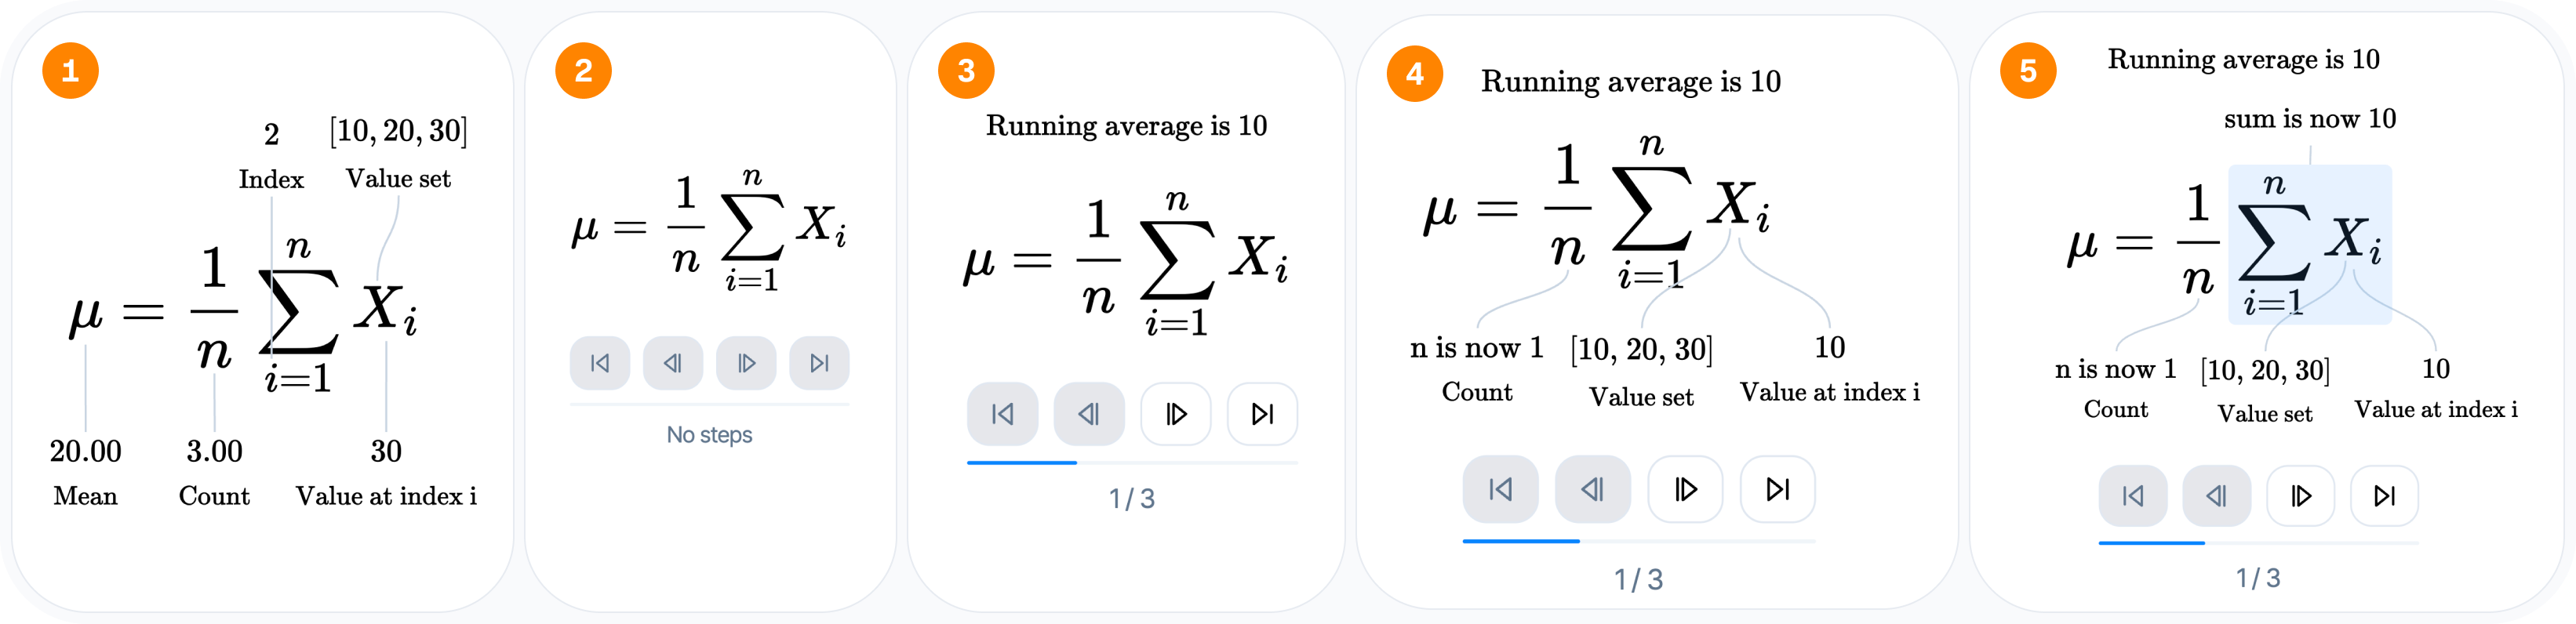
\includegraphics[width=\textwidth]{fig/demo-2.png}
  \caption{Average walkthrough authoring workflow. (1) Semantics produce final labels. (2) Stepping mode adds controls. (3) \texttt{step()} calls define pause points. (4) Labels anchor values to symbols. (5) LaTeX expression keys highlight notation spans.}
  \label{fig:demo-2}
\end{figure*}

Liv is now writing about the average formula $\mu = \frac{1}{n} \sum_{i=1}^{n} X_i$. She wants to walk students through the computation, showing how the running average evolves as each value is incorporated. She declares her formula and variables---including an array-valued variable \texttt{X}---and writes a semantics function that loops over the array:

\begin{tcolorbox}[codebox]
\begin{lstlisting}[style=jsstyle]
const config: Config = {
  formulas: [{
    id: "average",
    latex: "\\mu = \\frac{1}{n} \\sum_{i=1}^{n} X_i",
  }],
  variables: {
    "\\mu": { name: "Mean" },
    n: { name: "Count" },
    i: { name: "Index", precision: 0 },
    X_i: { name: "Value at index i", precision: 0 },
    X: { default: [10, 20, 30], name: "Value set" },
  },
  semantics: function ({ vars }) {
    vars.n = vars.X.length;
    var sum = 0;
    vars["\\mu"] = 0;
    for (var i = 0; i < vars.n; i++) {
      vars.i = i;
      vars.X_i = vars.X[i];
      sum = sum + vars.X_i;
      vars["\\mu"] = sum / (i + 1);
    }
    vars["\\mu"] = Math.round(vars["\\mu"] * 100) / 100;
  },
}
\end{lstlisting}
\end{tcolorbox}

With this configuration, the formula renders with labels showing the final computed values (Step~1 in Figure~\ref{fig:demo-2}). However, the loop executes all at once---the reader only sees the end result. To let students follow the computation one iteration at a time, Liv sets \texttt{stepping: true} and inserts \texttt{step()} calls inside the loop body. Each call marks a pause point and accepts a \texttt{description} and a \texttt{labels} object:

\begin{tcolorbox}[codebox]
\begin{lstlisting}[style=jsstyle]
stepping: true,
semantics: function ({ vars, step }) {
  ...
  for (var i = 0; i < vars.n; i++) {
    ...
    vars["\\mu"] = sum / (i + 1);
    step({
      description: "Running average is " + vars["\\mu"],
      labels: {
        "\\sum_{i=1}^{n} X_i": "sum is now " + sum,
        n: "n is now " + (i + 1),
        X_i: vars.X_i,
        X: vars.X,
      },
    });
  }
  vars["\\mu"] = Math.round(vars["\\mu"] * 100) / 100;
},
\end{lstlisting}
\end{tcolorbox}

With stepping enabled, Delta presents navigation controls (Step~2 in Figure~\ref{fig:demo-2}) rendered via a \texttt{StepControl} component. If \texttt{step()} calls are added in the semantics, by clicking forward, the display updates according to the step. (Step~3 in Figure~\ref{fig:demo-2}). Each key in the \texttt{labels} object is either a variable identifier or a LaTeX expression from the formula. Variable keys display values as labels beneath their symbol (Step~4 in Figure~\ref{fig:demo-2}); LaTeX expression keys highlight the corresponding notation span and attach the label to it (Step~5 in Figure~\ref{fig:demo-2}). At the first step, the summation span highlights with ``sum is now 10,'' $n$ shows ``n is now 1,'' and $X_i$ displays 10.  Students can trace the full trajectory of the running average, seeing how each new value shifts the mean, all without leaving the formula.